\documentclass[14pt]{extreport}
\usepackage{gost}
\usepackage{listings}

\begin{document}
\includepdf[pages={1}]{titul.pdf}

\newcommand\scalemath[2]{\scalebox{#1}{\mbox{\ensuremath{\displaystyle #2}}}}

% Математическое моделирование течений мелкой воды методом конечных элементов


\tableofcontents

\intro


// ОБОЗНАЧЕНИЯ И СОКРАЩЕНИЯ

Выполненная выпускная квалификационная работа посвящена задаче течения жидкости в озере, для которой требуется составить и решить систему дифференциальных уравнений с использованием метода конечных элементов (МКЭ). Предполагается, что глубина озера постоянна, а сам озеро однородно. Необходимо учесть, что озеро подвержено влиянию ветра, а так же требуется рассмотреть данную задачу с различными параметрами и проанализировать полученные результаты.

На данный момент во многих случаях не оправдывается применение более сложных математических моделей для исследования течений в прибрежных водах и озерах, чем моделей, основанных на численном решении двумерных уравнений, полученных путем применения осредненных по вертикали характеристик - уравнений мелкой воды. Трехмерные решения нецелесообразны, так как они требуют намного большего количества исходной информации и машинного времени даже с учетом современных вычислительных мощностей.

Целью представленной выпускной квалификационной работы является осуществление математического моделирования течений мелкой воды с помощью метода конечных элементов, который уже давно зарекомендовал в таких областях как механика деформируемого тела, электродинамика и конечно же гидродинамика. Данный метод является оптимальным для решения поставленной задачи так как именно он дает возможность применять достаточно гибкую разбивку рассматриваемой области и при его использовании достаточно удовлетворить лишь главным граничным условиям.

Актуальность данной работы обусловлена тем, что со второй половины 20-го века метод математического моделирования стал рабочим инструментом при изучении многих научно-технических задач, в частности, и в области гидродинамики. Основной составляющей этого метода стал является вычислительных эксперимент, широкое применение которого стало возможным благодаря развитию производительности ЭВМ и численных алгоритмов. Вычислительный эксперимент позволяет получить информацию о структуре течения при относительно небольших временных, трудовых и материальных затратах. конечно, при этом соответствующая математическая модель должна быть адекватной физическому процессу.

Научная новизна работы заключается в применении МКЭ конкретно к уравнениям мелкой воды и составлении программной реализации на языке программирования Python.

В данной работе будут представлены основные определения и понятия для уравнений мелкой воды, которые позволят составить и решить поставленную задачу, которая состоит из двух частей: аналитической и численной. Аналитически будут описаны течения жидкости при пренебрежении температурными эффектами, для которых широко используются классические уравнения Сен-Венана. После этого с помощью МКЭ будет построена и рассчитана математическая модель. Для реализации такой модели была написана программа, которая выдает результаты решения системы уравнений мелкой воды, а так же генерирует графики, которые наглядным образом отображают полученные результаты.

\chapter{Уравнения мелкой воды}

Запишем два основных уравнения для жидкости. Это уравнение количества движения и уравнение неразрывности \cite{Konor:1979:FEM}:

\begin{gather}
-\frac{\partial p}{\partial x_k} + \frac{\partial \tau_{ik}}{\partial x_i} + \rho b_k = \frac{\partial}{\partial x_i}(\rho v_i v_k) + \frac{\partial}{\partial t}(\rho v_k);
\end{gather}.

\begin{gather}
\frac{D\rho}{Dt}+\rho \frac{\partial v_i}{\partial x_i} =0
\end{gather}

Если в (1.1) и (1.2) пренебречь температурными эффектами, получим:

\begin{gather}-\frac{\partial p}{\partial x_k} + \frac{\partial \tau_{ik}}{\partial x_i} + \rho b_k = \frac{D(\rho v_k)}{Dt}
\end{gather}

\begin{gather}\frac{\partial (\rho v_i)}{\partial t} + \frac{\partial \rho}{\partial t}=0,
\end{gather}

\noindentгде $ p $ - давление, оказываемое на единицу площади поверхности воды, $ b_k $ - массовые силы, приходящиеся на единицу массы, $v_k$ - скорость частицы воды в направлении оси $x_k$, $\tau_{ik}$ - вязкостные составляющие вектора напряжения, $ \rho $ - массовая плотность воды.

В задачах циркуляции воды сложно применять данные уравнения из-за наличия свободной поверхности, изменения границ во время приливов и отливов и вследствие большого количества переменных.

Данные трудности могут быть упрощены, в результате чего получается уравнения мелкой воды. Первое упрощение состоит в том, что уравнение количества движения в проекции на ось $ x_3 $ записывается в виде:

\begin{gather}
-\frac{\partial p}{\partial x_3}=\rho g, 
\end{gather}

\noindentгде массовые силы отрицательны, поскольку действуют в направлении противоположном оси $ x_3 $. При выводе формулы (1.5) пренебрегаем всеми членами, которые характеризуют ускорение и соответствующими им напряжениям. Проинтегрируем выражение (1.5), и в результате получим:

\begin{gather}
p = \int\limits^\eta_{x_3} \rho g dx_3 = \rho g (\eta-x_3)+p_a,
\end{gather}

\noindent где $p_a$ атмосферное давление на поверхности воды
$\eta$ - возвышение свободной поверхности в соответствии с рисунком 1.1.

%\begin{figure}[H]
%\centerline{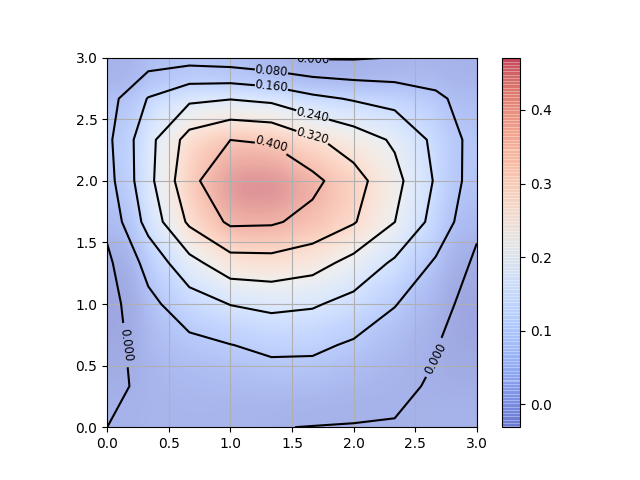
\includegraphics[width=0.5\linewidth]{1}}
%\caption{Определение типов границы}
%\label{fig11}
%\end{figure}


Оставшиеся два уравнения количества движения по направлениям $x_1$ и $x_2$ останутся без изменений:

\begin{gather}
-\frac{\partial p}{\partial x_k} + \frac{\partial \tau_{ik}}{\partial x_i} + \rho b_k = \frac{D(\rho v_k)}{Dt}.
\end{gather}

\noindentПри $k=1$ выражение (1.7) дает проекцию на ось $ x_1 $ , при $k=2$ - на ось $ x_2 $. В выражении (1.7) величина $v$ есть средняя скорость, $\rho$ - переменная массовая плотность и $\tau$ - сумма вязкостных и турбулентных напряжений.

Проинтегрируем выражения (1.4) и (1.7) по $ x_3 $. Для уравнения неразрывности это даст:

\begin{gather}
\int\limits^\eta_{-h} \bigg(\frac{\partial (\rho v_i)}{\partial x_i} + \frac{\partial \rho}{\partial t}\bigg) dx_3 =0,
\end{gather}

\noindentгде $h$ - это глубина измеряемая от базовой поверхности (в общем случае не горизонтальной).

Определим поток $ q_k $ количества жидкости (массу жидкости, приходящуюся на единицу длины и времени):


\begin{gather}
q_i = \int\limits^\eta_{-h} \rho v_i dx_3 = \rho \int\limits^\eta_{-h} v_i dx_3,
\end{gather}

\noindentПредполагается, что $\rho(x_1, x_2)$ не зависит от $x_3$.

При интегрировании уравнения (1.8) необходимо использовать кинематическое условие и правило Лейбница \cite{Zorich:2002:CALC} для вычисления частной производной интеграла с переменными пределами. Согласно этому правилу:


\begin{gather}
\frac{\partial}{\partial x_1} \int\limits^{h_2(x_1,x_2)}_{h_1(x_1,x_2)} f(x_1, x_2, x_3) dx_3=\int\limits^{h_2(x_1,x_2)}_{h_1(x_1,x_2)} \frac{\partial f}{\partial x_1} dx_3 + f \bigg|_{h_2}  \frac{\partial h_2}{\partial x_1} + f \bigg|_{h_1} \frac{\partial h_2}{\partial x_1};
\end{gather}

\noindent(аналогично для производной по $x_2$).

Кинематическое соотношение для свободной поверхности можно записать как:

\begin{gather}
v_3\bigg|_{x_2=\eta} = \frac{D\eta}{Dt} = \frac{\partial \eta}{\partial t} + v_1 \bigg|_{\eta} \frac{\partial \eta}{\partial x_1} + v_2 \bigg|_{\eta}\frac{\partial \eta}{\partial x_2}
\end{gather}

Применим формулы (1.9)-(1.11) к уравнению (1.8), и получим:

\begin{gather}
\frac{ \partial q_i}{\partial x_i} + \frac{\partial(\rho H)}{\partial t} = 0,
\end{gather}

\noindentгде $H=\eta+h $.

Чтобы проинтегрировать уравнение количества движения (1.7) по $x_3$, определим мгновенные скорости $v_1$, $v_2$:

\begin{gather}
v_1 = \overline{v_1} (x_1, x_2, t) + v_1'(x_1, x_2, x_3, t); \nonumber\\
v_2 = \overline{v_2} (x_1, x_2, t) + v_2'(x_1, x_2, x_3, t), \end{gather}

\noindentгде величина $\overline{v}$ означает средние по вертикали скорости, а $v’$ - отклонение от этих средних значений при различных значениях $x_3$.

Следовательно:

\begin{gather}
<v_k>=\int\limits^\eta_{-h} v_k dx_3 = \frac{1}{\rho} q_k, \; v_k=\frac{1}{H}<v_k>,
\end{gather}

\noindentТак как $ <v_k’> = 0 $, где знак $ <> $ означает среднее значение стоящий внутри величины.

Будем предполагать, что массовые силы обусловлены только эффектом Кориолиса. Таким образом:

\begin{gather}
b_1 = \rho f v_2, \; b_2 = - \rho f v_1.
\end{gather}
\noindentПредположим, что наклоны поверхности и дна малы по сравнению с единицей, тогда составляющие внутреннего напряжения можно аппроксимировать следующим образом:

\begin{gather}
 \tau_1\bigg|_s \approx \bigg\{ -\tau_{11}\frac{\partial \theta}{\partial x_1} -\tau_{12}\frac{\partial \theta}{\partial x_2} +\tau_{13}\bigg\}, \nonumber \\
\tau_1\bigg|_b \approx \bigg\{ \tau_{11}\frac{\partial h}{\partial x_1} +\tau_{12}\frac{\partial h}{\partial x_2} -\tau_{13}\bigg\},
\end{gather}

\noindentАналогичные значения можно выписать для величин $\tau_2|_s$ и $\tau_2|_b$.

Величины $\tau_2|_s$ и $\tau_2|_b$ можно интерпретировать как компоненты внешней силы, приложенные к поверхности и ко дну.

Подставим теперь соотношения (1.13) - (1.15) в уравнение количества движения, проинтегрированные по $x_3$ и дополнительно используем правило Лейбница и кинематическое условие. Тогда:

\begin{gather} 
\frac{\partial q_1}{\partial t} + \frac{\partial}{\partial x_1} \bigg(\frac{q_1^2}{H}\bigg)+\frac{\partial }{\partial x_2}\bigg(\frac{q_1 q_2}{H}\bigg) = -\frac{\partial N_p}{\partial x_2} + \frac{\partial N_{11}}{\partial x_1} + \frac{\partial N_{12}}{\partial x_2} \nonumber\\+ fq_2 + p\bigg|_s \frac{\partial \eta}{\partial x_1} + \tau_1\bigg|_s+p\bigg|_b\frac{\partial h}{\partial x_1} - \tau_1\bigg|_b;  \nonumber\\
\frac{\partial q_2}{\partial t} + \frac{\partial}{\partial x_1} \bigg(\frac{q_1 q_2}{H}\bigg)+\frac{\partial }{\partial x_2}\bigg(\frac{q_2^2}{H}\bigg) = -\frac{\partial N_p}{\partial x_2} + \frac{\partial N_{22}}{\partial x_2} + \frac{\partial N_{21}}{\partial x_1} \nonumber\\+ fq_1 + p\bigg|_s \frac{\partial \eta}{\partial x_2} + \tau_2\bigg|_s+p\bigg|_b\frac{\partial h}{\partial x_2} - \tau_2\bigg|_b,
\end{gather}

\noindentгде

\begin{gather} 
N_p = <p> = \int\limits^\eta_{-h} pdx_3=\rho g \frac{H^2}{2} + Hp_a; \nonumber\\
N_{11} = <\tau_{11}>-<pv_1'v_1'>; \nonumber\\
N_{22} = <\tau_{22}>-<pv_2'v_2'>; \nonumber\\
N_{12} = <\tau_{12}>-<pv_1'v_2'>;
\end{gather}

\noindentБолее того, элементы $N_{ik}$ могут быть аппроксимированы следующими выражениями:

\begin{gather} 
N_{11} \approx 2 \varepsilon_{11}\frac{\partial q_1}{\partial x_1}; \nonumber\\
N_{22} \approx 2 \varepsilon_{22}\frac{\partial q_2}{\partial x_2}; \nonumber\\
N_{12} \approx \varepsilon_{12}\bigg(\frac{\partial q_2}{\partial x_1}+\frac{\partial q_1}{\partial x_2}\bigg);
\end{gather}


\noindentгде $\varepsilon_{ik}$ обобщенные коэффициенты вихревой вязкости. Для изотропного характера течения $\varepsilon_{11}=\varepsilon_{22}=\varepsilon_{12}=\varepsilon.$

Касательные напряжения на дне обычно определяются соотношениями:

\begin{gather}
\tau_1\bigg|_b = \frac{g}{c^2} \frac{1}{\rho} \frac{q_1\sqrt{(q_1^2+q_2^2)}}{H^2}; \nonumber\\
\tau_2\bigg|_b = \frac{g}{c^2} \frac{1}{\rho} \frac{q_2\sqrt{(q_1^2+q_2^2)}}{H^2};
\end{gather}

\noindentгде $g$ - ускорение силы тяжести, $с$ - коэффициент трения, $\rho$ - плотность воды. 

Составляющие напряжения трения на поверхности воды обычно обусловлены действием ветра и могут быть найдены по формулам:

\begin{gather}
\tau_1\bigg|_s=\gamma^2\rho_aW^2\cos(\Theta); \nonumber\\
\tau_2\bigg|_s=\gamma^2\rho_aW^2\sin(\Theta);
\end{gather} 

\noindentгде $\gamma^2$ - коэффициент ветрового напряжения, $\rho_a$ - плотность воздуха, $W$ - скорость ветра, $\theta$ - угол между осью $x_1$ и направлением ветра.

Уравнения (1.17) перепишем в виде:


\begin{eqnarray} 
\frac{\partial q_1}{\partial t} + \frac{\partial}{\partial x_1} \bigg(\frac{q_1^2}{H}\bigg)+\frac{\partial }{\partial x_2}\bigg(\frac{q_1 q_2}{H}\bigg) = \frac{\partial}{\partial x_1} (N_{11}-N_p) + \frac{\partial N_{12}}{\partial x_2} + B_1; \nonumber\\
\frac{\partial q_2}{\partial t} + \frac{\partial}{\partial x_1} \bigg(\frac{q_1 q_2}{H}\bigg)+\frac{\partial }{\partial x_2}\bigg(\frac{q_2^2}{H}\bigg) = \frac{\partial}{\partial x_2} (N_{22}-N_p) + \frac{\partial N_{12}}{\partial x_2} + B_2,
\end{eqnarray}

\noindentгде

\begin{eqnarray}
B_1=fq_2+\gamma^2\rho_aW^2\cos(\Theta)-\bigg(\frac{g}{c^2}\bigg)\frac{1}{\rho}\frac{q_1\sqrt{(q_1^2+q_2^2)}}{H^2} + p_a \frac{\partial H}{\partial x_1} + \rho gH\frac{\partial h}{\partial x_1}; \nonumber\\
B_2=-fq_1+\gamma^2\rho_aW^2\sin(\Theta)-\bigg(\frac{g}{c^2}\bigg)\frac{1}{\rho}\frac{q_2\sqrt{(q_1^2+q_2^2)}}{H^2} + p_a \frac{\partial H}{\partial x_2} + \rho gH\frac{\partial h}{\partial x_2}.
\end{eqnarray}

Для решения окончательной системы уравнений (1.22), дополненных условием (1.12) необходимо установить требуемые граничные условия. Будем считать, что граница $S$ состоит из двух частей: твердой границы $S_1$ и жидкой $S_2$, представляющей границу рассматриваемого водоема с открытым морем в соотвествии с рисунком 1.2.

\begin{figure}[H]
\centerline{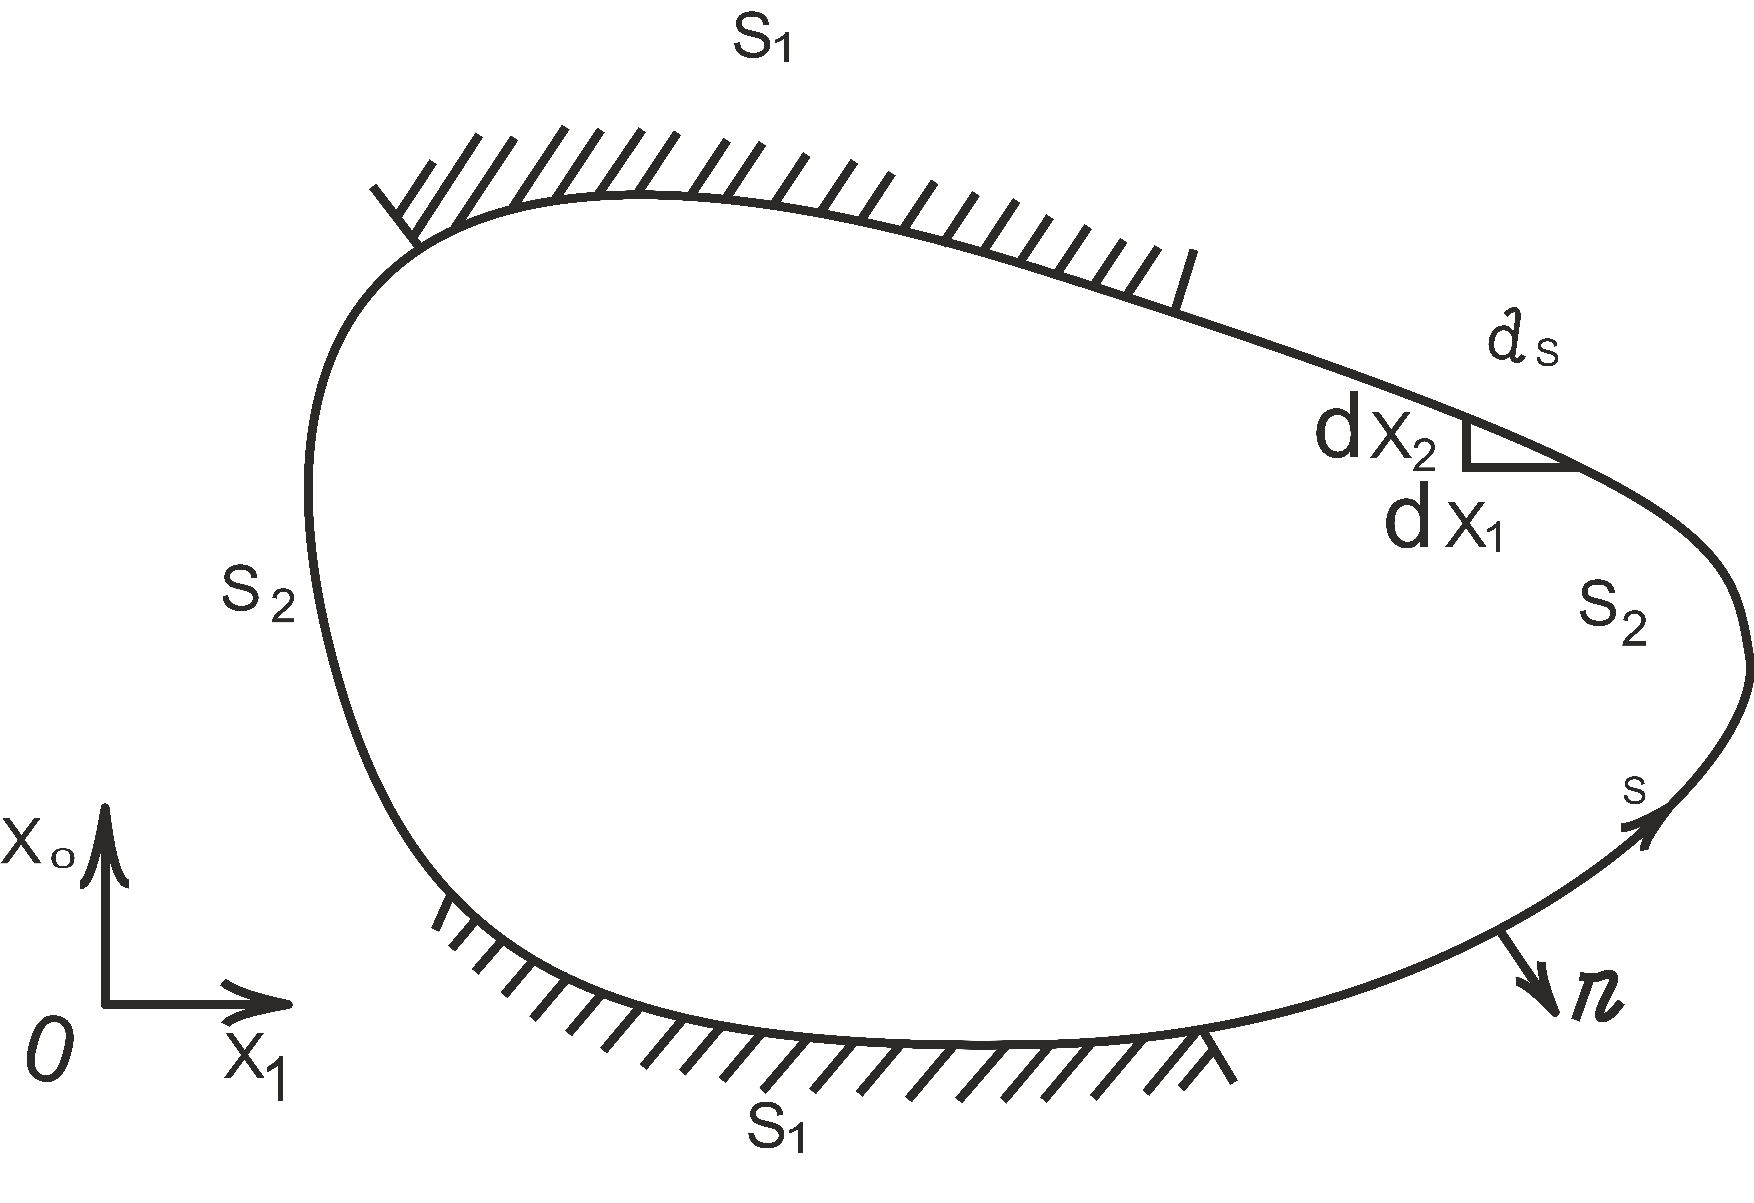
\includegraphics[width=0.5\linewidth]{2}}
\caption{Определение типов границы}
\label{fig11}
\end{figure}

В системе координат $s-n$ связанной с границей течения, расход массы жидкости можно записать через $q_s$ и $q_n$:

\begin{eqnarray}
q_n=\int\limits^\eta_{-h} \rho v_n dx_3= \alpha_{n1}q_1+\alpha_{n2}q_2; \nonumber\\
q_s=\int\limits^\eta_{-h} \rho v_s dx_3= -\alpha_{n2}q_1+\alpha_{n1}q_2;
\end{eqnarray}

\noindentгде $\alpha_{n1}=\cos(\overline{n},x_1); \alpha_{n2}=\cos(\overline{n},x_2).$

Для установления результирующих сил можно воспользоваться формулами:

\begin{eqnarray}
N_{n1}=\alpha_{n1}(N_{11}-N_{p})+\alpha_{n2}N_{12}; \nonumber\\
N_{n2}=\alpha_{n1}N_{12}+\alpha_{n2}(N_{22}-N_{p}).
\end{eqnarray}

По значениями $N_{n1}$ и $N_{n2}$ определяется нормальная и касательная составляющая результирующей силы для наклонной площадки:

\begin{eqnarray}
N_{nn}=\alpha_{n1}N_{n1}+\alpha_{n2}N_{n2}; \nonumber\\
N_{ns}=\alpha_{n2}N_{n1}+\alpha_{n1}N_{n2}.
\end{eqnarray}

Если же в исследуемую акваторию впадает река, то на $ S_1 $:

\begin{eqnarray}
q_n=\overline{q_n}=|q|; \nonumber\\
q_s=0.
\end{eqnarray}

\noindentгде $|q|$ - поток втекающей
реки. 

На жидкой границе $ S_2 $ необходимо задать нормальные и касательные силы:

\begin{eqnarray}
N_{nn}=\overline{N_{nn}}; \nonumber\\
N_{ns}=\overline{N_{ns}}.
\end{eqnarray}

\noindentНо так как слагаемыми, учитывающими вихревую вязкость в уравнении (1.22) можно пренебречь, то касательные силы или скорости не могут быть заданы. Таким образом граничные условия сводятся к следующим:

\begin{eqnarray}
q_n=0 \; \text{или} \; q_n=\overline{q_n} \; \text{на} \; S_1\nonumber\\
N_{nn}=\overline{N_{nn}}=-N_p \; \text{на} \; S_2.
\end{eqnarray}


// TODO

Уравнение (1.37) вместе с граничными условиями (1.39) допускает вариационную формулировку и применение метода конечных элементов.










\chapter{Постановка задачи}

Пусть дана система уравнений мелкой воды, описываемая уравнениями ()-(), которые были выведены в первой главе:

// тут будут уравнения

где

// перечисляю параметры


Так же даны какие-то начальные условия

// условия


Для начала данные уравнения будут переписаны в терминах методы конечных элементов, а после будет составлен алгоритм и написана программная реализация МКЭ для системы (которая выше).


\chapter{Триангуляция двумерной области}

В геометрии триангуляция в наиболее общем значении — это разбиение геометрического объекта на $N$ фигур, из которых одна является внешней неограниченной, о остальные - симплексами -  геометрические фигуры, которые являются $n-$мерным обобщением треугольника. 


Алгоритмические исследования задачи построения триангуляции появились в научной
литературе во второй половине XX века. Систематическое изучение геометрических
алгоритмов было предпринято в середине 70-х г. [ Препарата Ф., Шеймос М. Вычислительная геометрия: Введение. –– М.: Мир, 1989. ––
478 с.]


Триангуляция дискретного множества точек $P\subset {\mathbb  {R}}^{{n+1}}$ — это разбиение выпуклой оболочки точек на симплексы так, что:

	1. любые два симплекса в T пересекаются в общей грани ребра или вершины, или вообще не пересекаются;

	2. множество точек, являющихся вершинами симплексов разбиения, совпадает с множеством ${\displaystyle P}$. 

Наиболее известным видом триангуляции множества точек является триангуляция Делоне, но в общем виде для метода конечных элементов она не подходит по причине того, что двумерная область изначально будет определяться набором точек, которые характеризуют контур рассматриваемой области. С точки зрения классического алгоритма Делоне произвольный набор точек будет являться неоднозначным, выпуклым многоугольником. Для того, чтобы однозначно триангулировать область которая ограничена контуром будем применять алгоритм L. Paul Chew, который так же называют усовершенствованным алгоритмом Делоне


http://2011.cccg.ca/PDFschedule/papers/paper91.pdf





\chapter{Метод конечных элементов в двумерной области}









\chapter{Учёт граничных условий}
\chapter{Изменение формы водоёма (прямоугольник, круг, реальный водоём)}
\chapter{Учёт наличия острова (островов) внутри водоёма}

// тут рассмотрим сетку


\chapter{Разработка базы данных для хранения информации о проведённых экспериментах}


\bibliographystyle{ugost2008}
\bibliography{biblio}


\end{document}
2